\section{Results}

\subsection{Previous literature suggested a T cell-mediated autoimmune disorder of the hematopoietic system.}

Among all the 513 search results, there are 43 articles about aplastic anemia involves certain bioinformatics analysis, ranging from sequence comparison to transcriptomics analysis. 

All the 43 articles mentioned autoimmune disorder in most aplastic anemia cases, while 12 of them gives us an insight that T cell-mediated autoimmune disorder is closely related to aplastic anemia. Immune-mediated destruction of hematopoietic stem and progenitor cells is pathophysiologic in most cases of aplastic anemia (AA).\cite{zeng2004transcript}

The generated word cloud plot is shown below.

\begin{figure}[H]
    \centering
    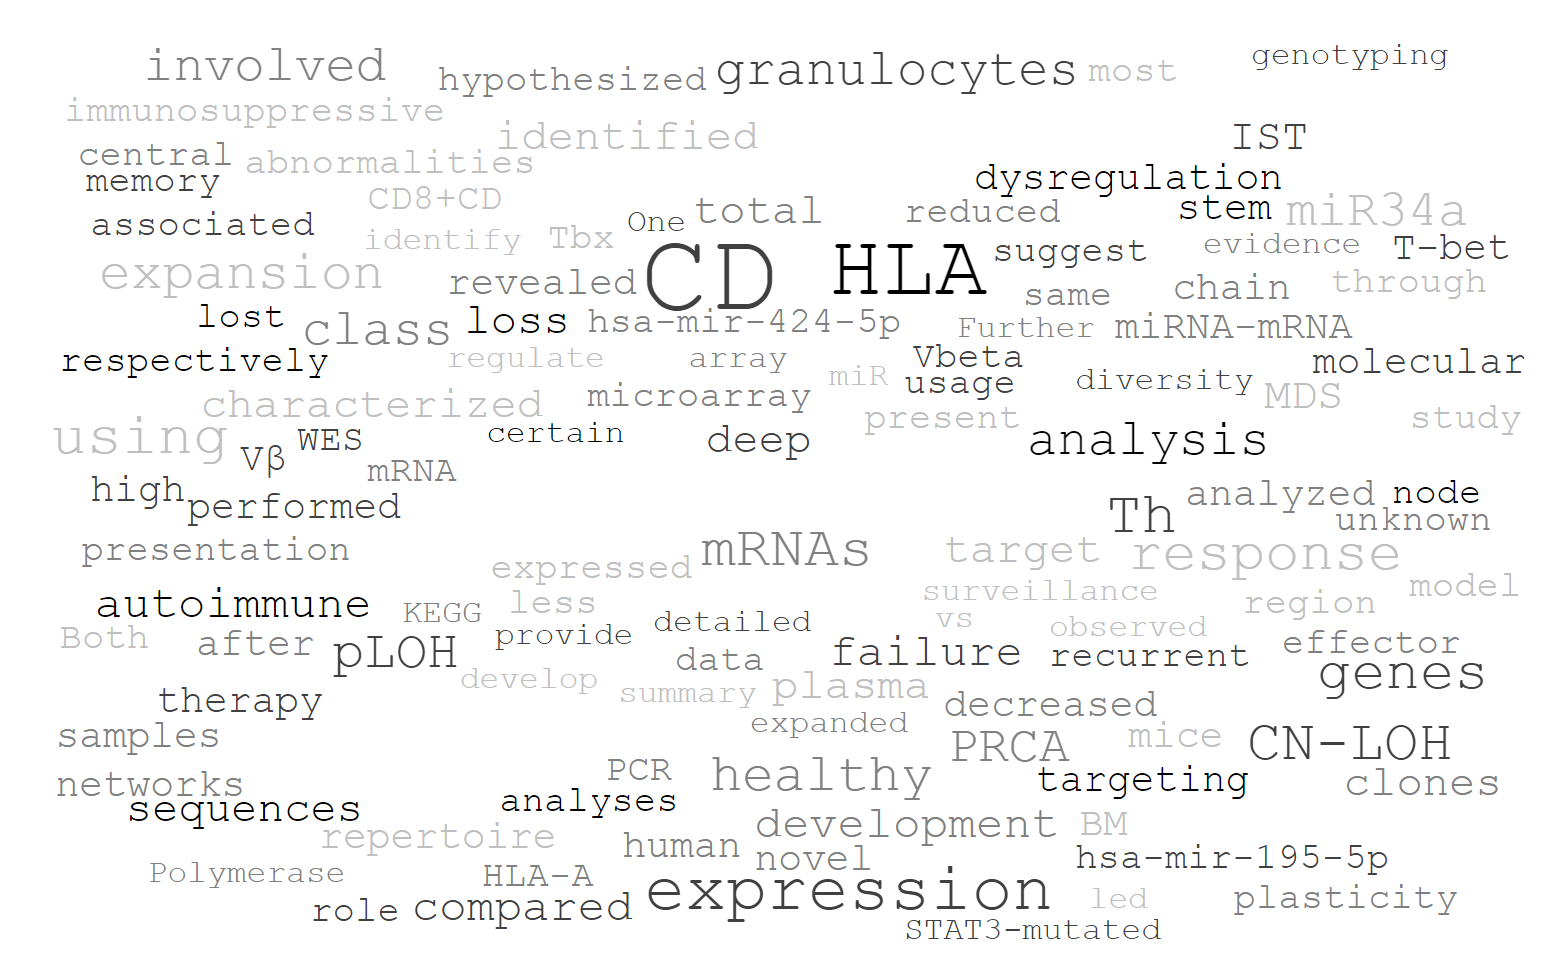
\includegraphics[width=0.6\textwidth]{image/wordcloud.png}
    \caption{Selection standard}
    \label{WORD}
\end{figure}

We selected several articles involving the bioinfomatics skills we have learnt in this course as our data source to perform our analysis. The selected articles are listed in Supplementary Material section.


\subsection{Transcriptomics analysis of CD3+ T-cell reveals that platelet factor 4 is related to aplastic anemia pathophysiology.}

We fetched the data set GSE3807 from GEO. The data set is collected from 8 volunteers using Affymetrix Human Genome U133A Array (GPL96). Among the 8 samples, 6 are suffering from aplastic anemia, while the other 2 samples are from healthy control.\cite{franzke2006identification}

We identified the top 250 differently expressed genes from the data set, with the worst p value of 0.011. Using the differently expressed genes, we did a principal component analysis, and the result is shown below.

\begin{figure}[H]
    \centering
    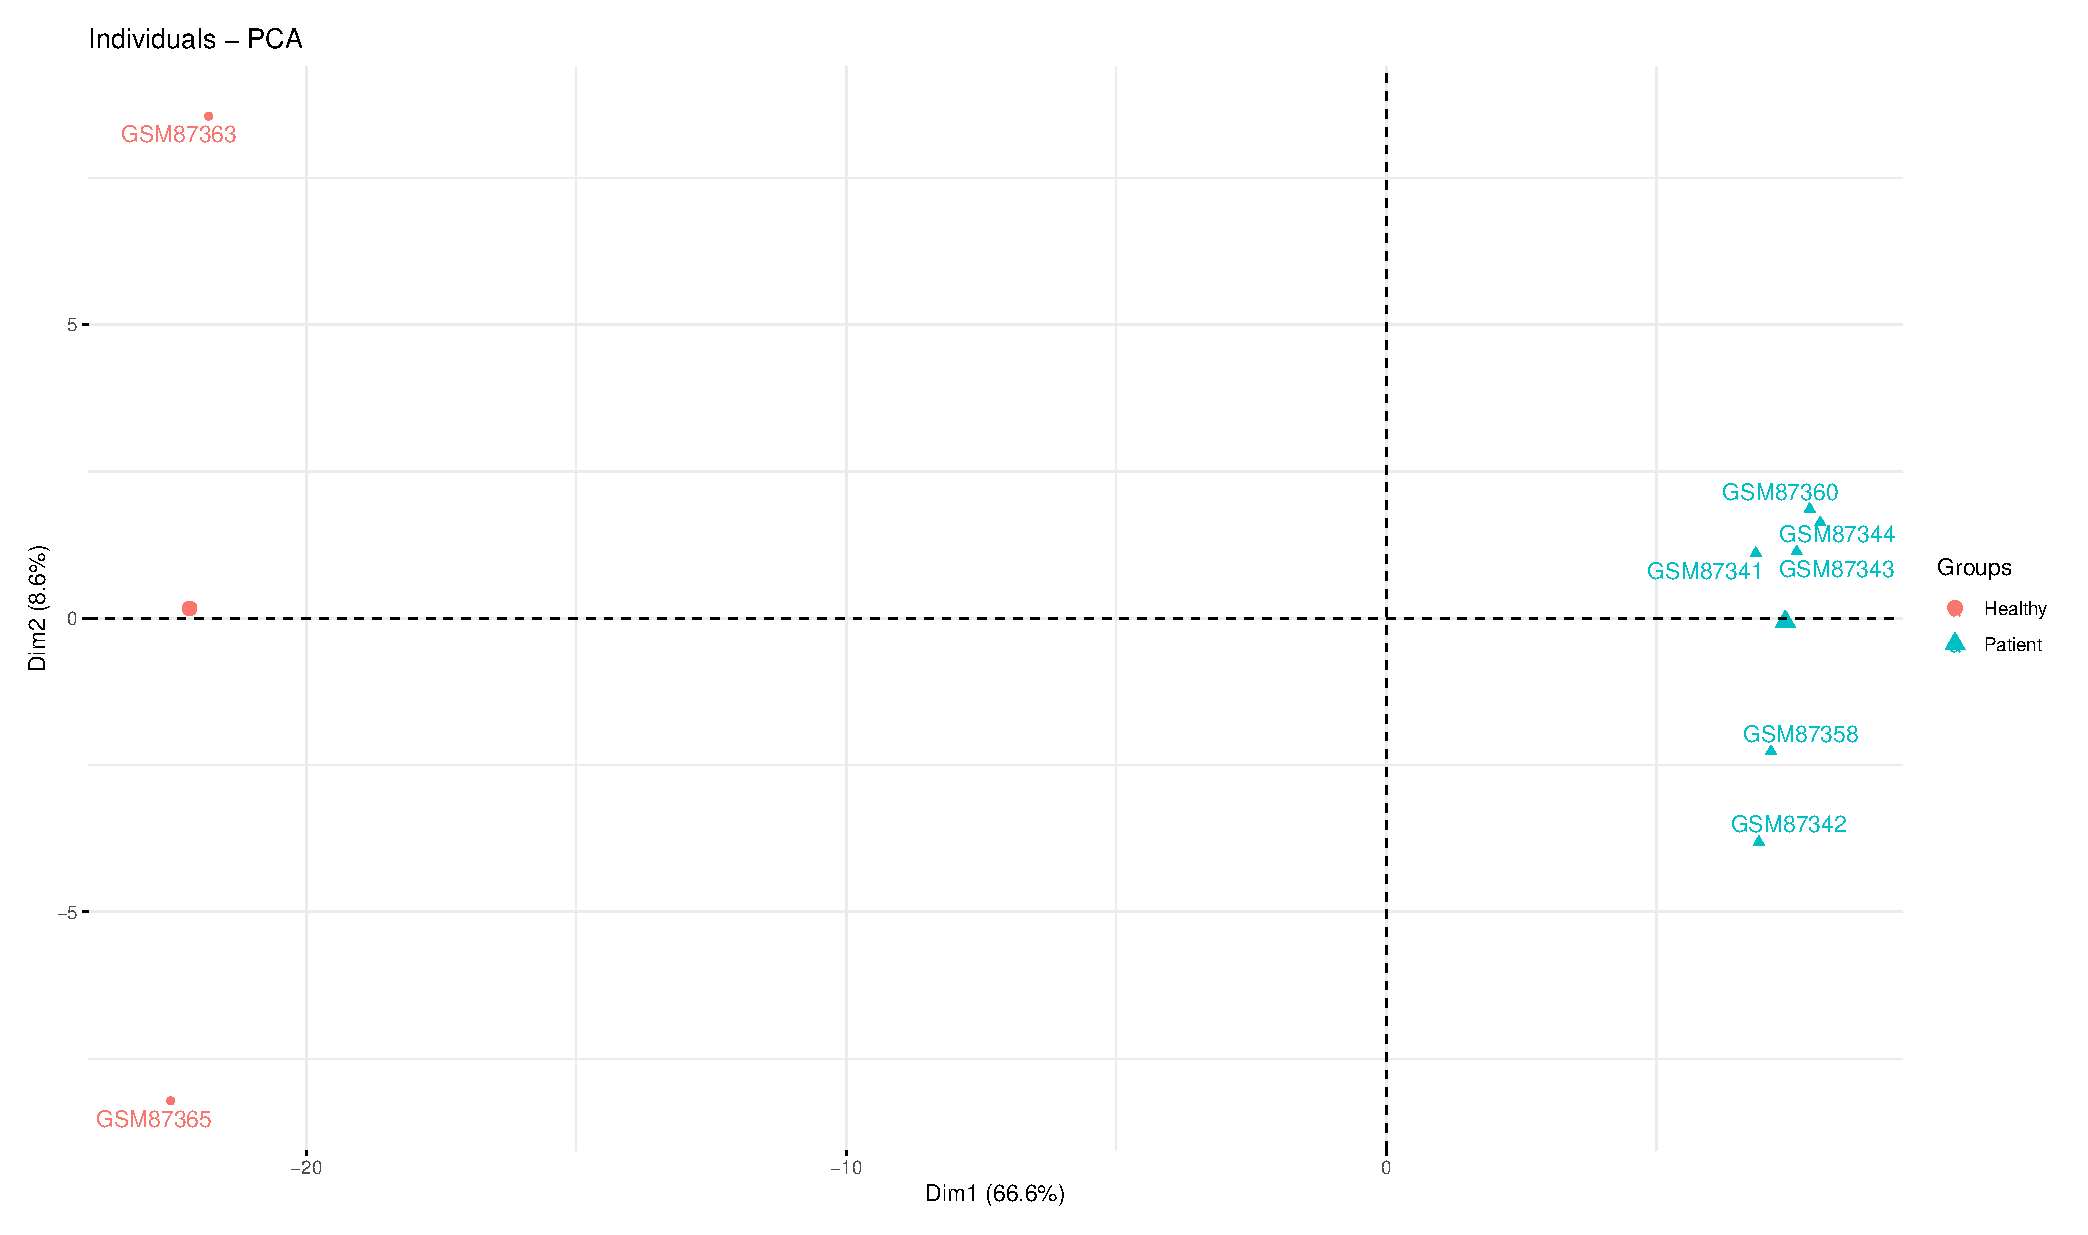
\includegraphics[width=0.9\textwidth]{image/PCACD31.eps}
    \caption{Result of principal component analysis}
    \label{PCACD3}
\end{figure}

PC1 and PC2 consist over 70\% of the principal components, which indicates that the analysis is desirable. According to the figure above, two groups of people are well separated by the PC1 and PC2 of the principal component analysis algorithm.

\begin{figure}[H]
    \centering
    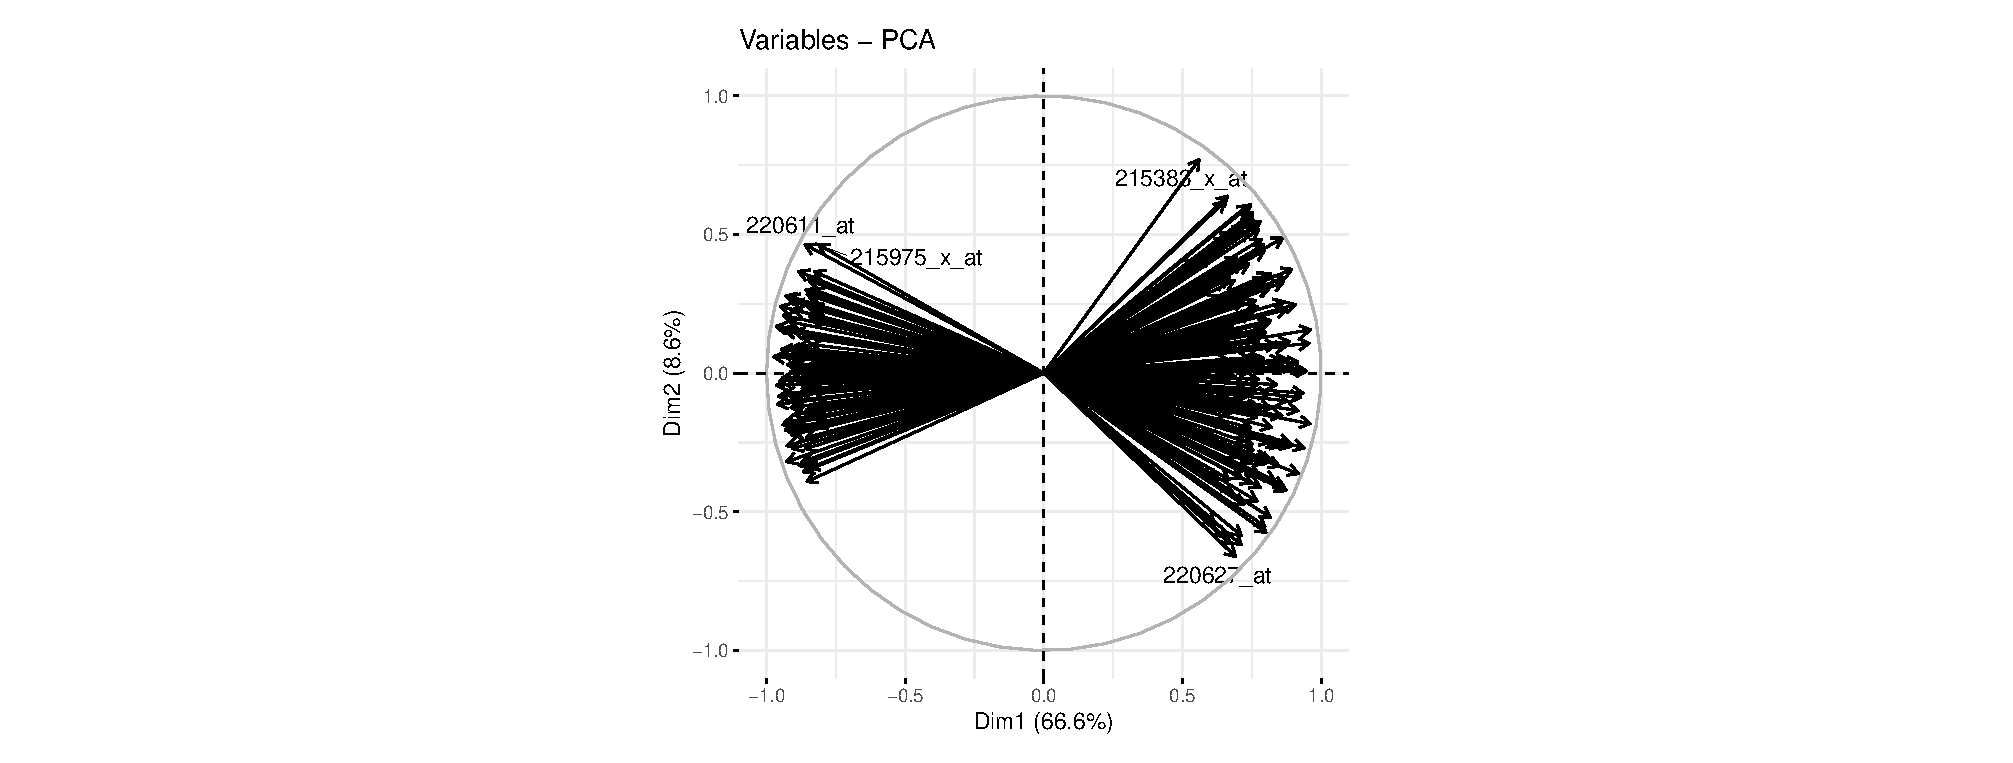
\includegraphics[width=0.5\textwidth]{image/PCAVCD3.eps}
    \caption{Variance of principal component analysis}
    \label{PCACD3}
\end{figure}


Heat map of the differently expressed genes is shown below.

\begin{figure}[H]
    \centering
    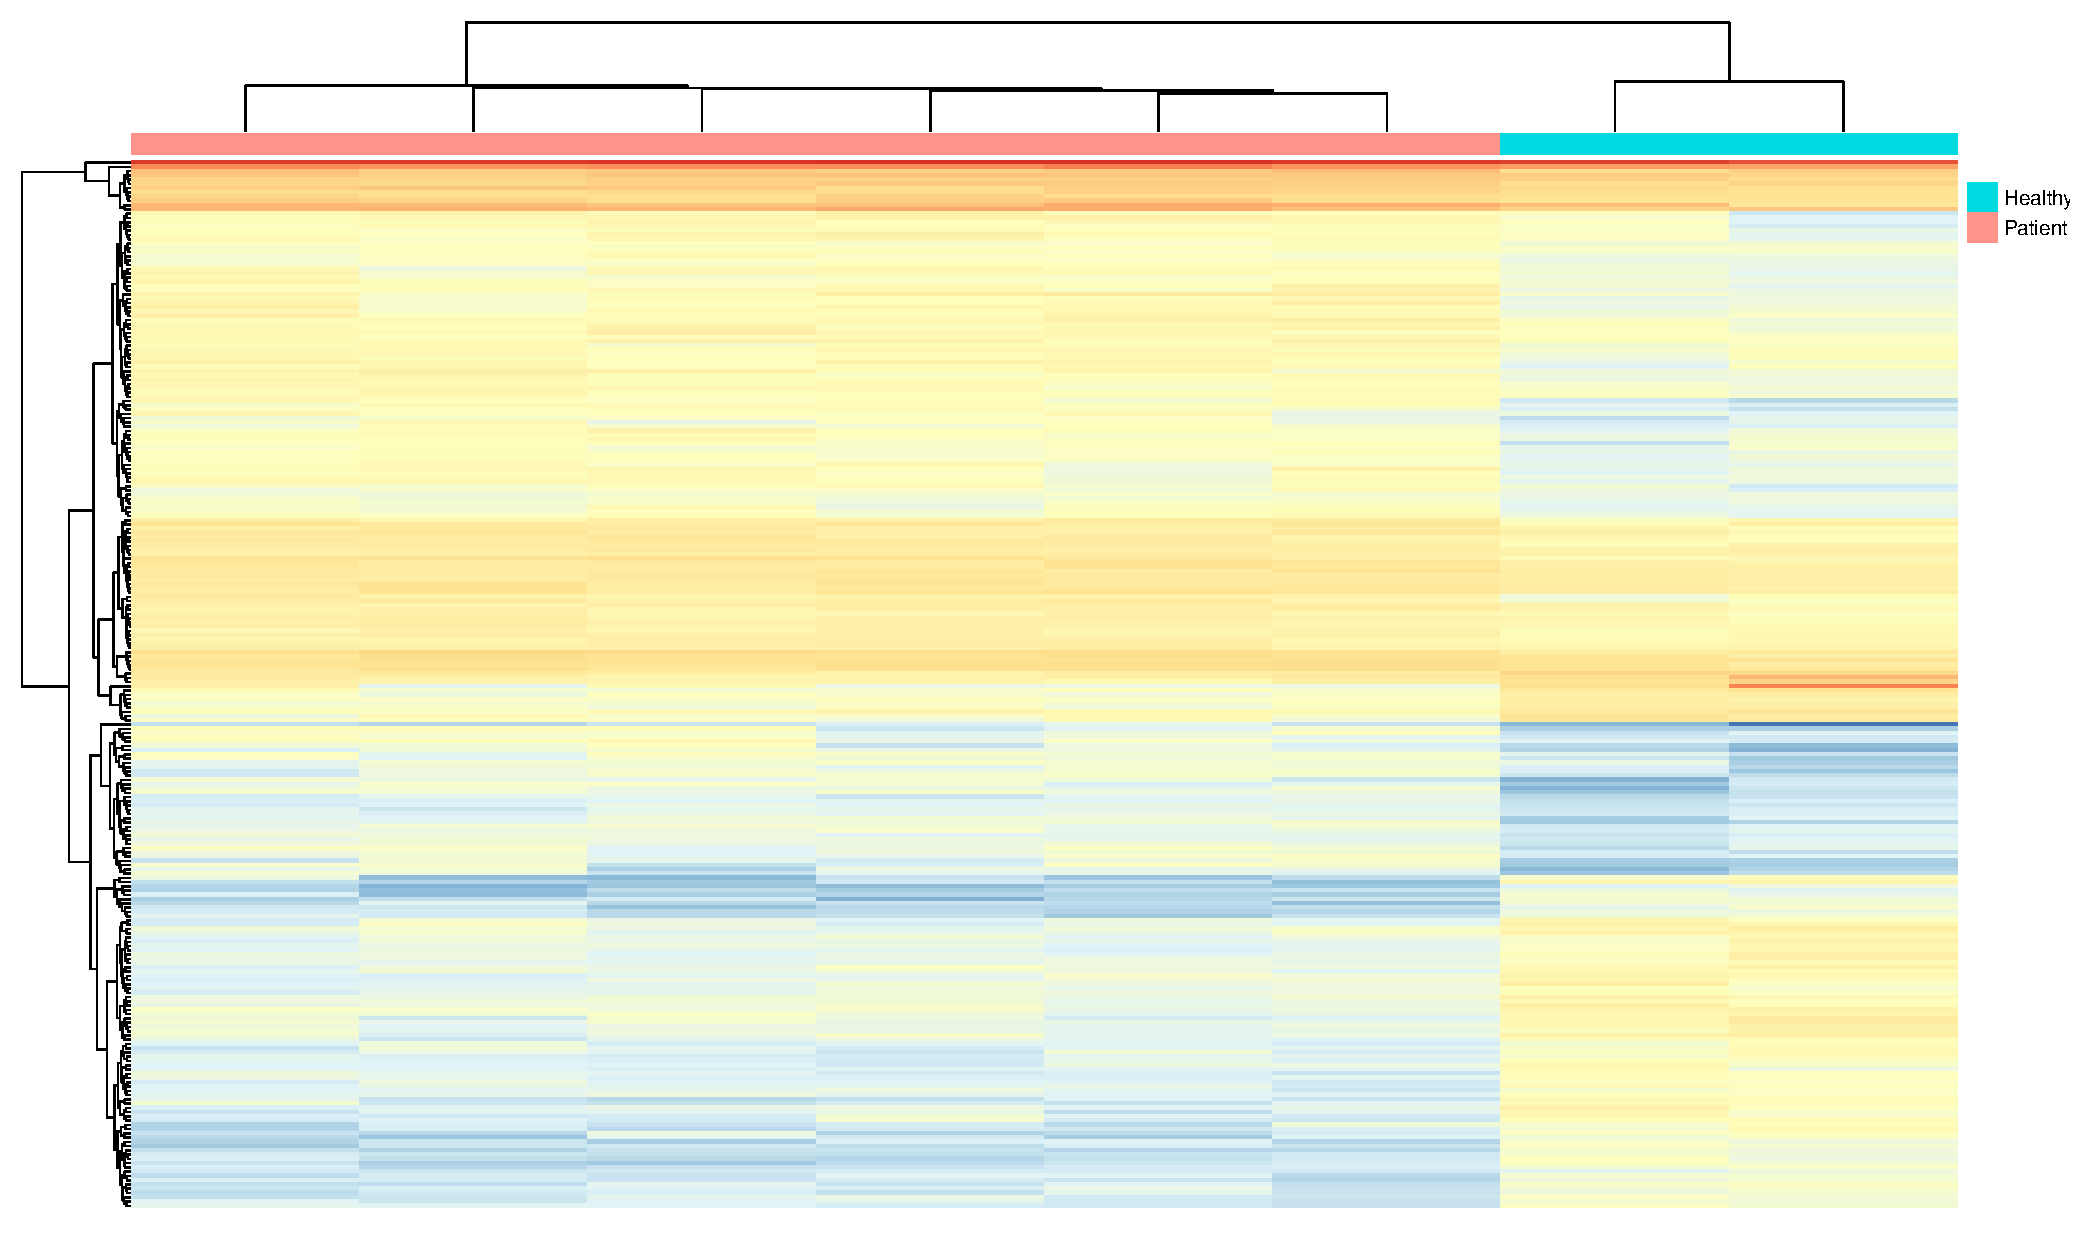
\includegraphics[width=0.9\textwidth]{image/HMCD3.eps}
    \caption{Heat map of the differently expressed genes}
    \label{HMCD3}
\end{figure}

From the heat map and the clustering results, clear divergence can be seen between the two groups. The main difference of the two groups are the genes that are down regulated in the Patients group, which is the lower-left part of the heat map.

To find out the functions of the down regulated genes, we did a GO enrichment on all down regulated genes, and the resulting dot plot is shown below.

\begin{figure}[H]
    \centering
    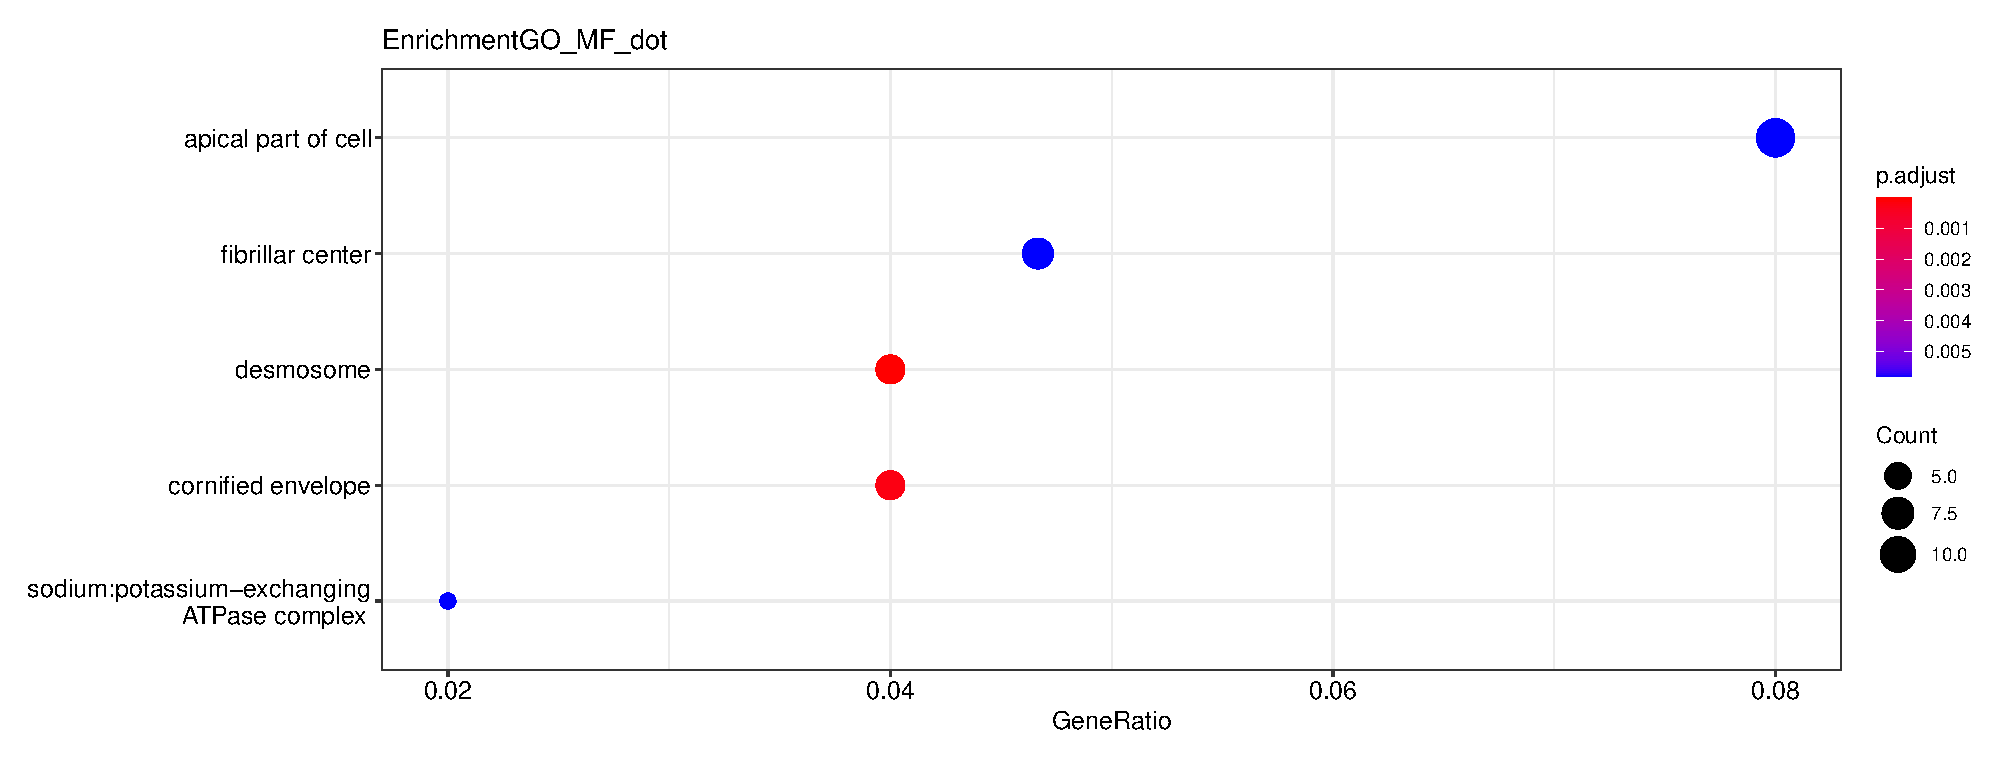
\includegraphics[width=1\textwidth]{image/EGOCD3.eps}
    \caption{GO enrichment of down regulated genes}
    \label{HMCD3}
\end{figure}

Among the down regulated genes, one gene named platelet factor 4 (PF4) caught our attention. PF4 is 27 folds lower in the patients group than in healthy control, and the p value of the gene is 0.005. Considering that PF4 is closely related to platelet formation and functions, we can say that platelet factor 4 is related to aplastic anemia pathophysiology.

\subsection{Platelet factor 4 has sequence homology with some chemokine family members.}

We fetched the sequence of Platelet factor 4, and run a psi-blast against the NCBI protein database, and the organism is limited to human. The results are then analysed using ClustalX 2.1 to perform an MSA.

\begin{figure}[H]
    \centering
    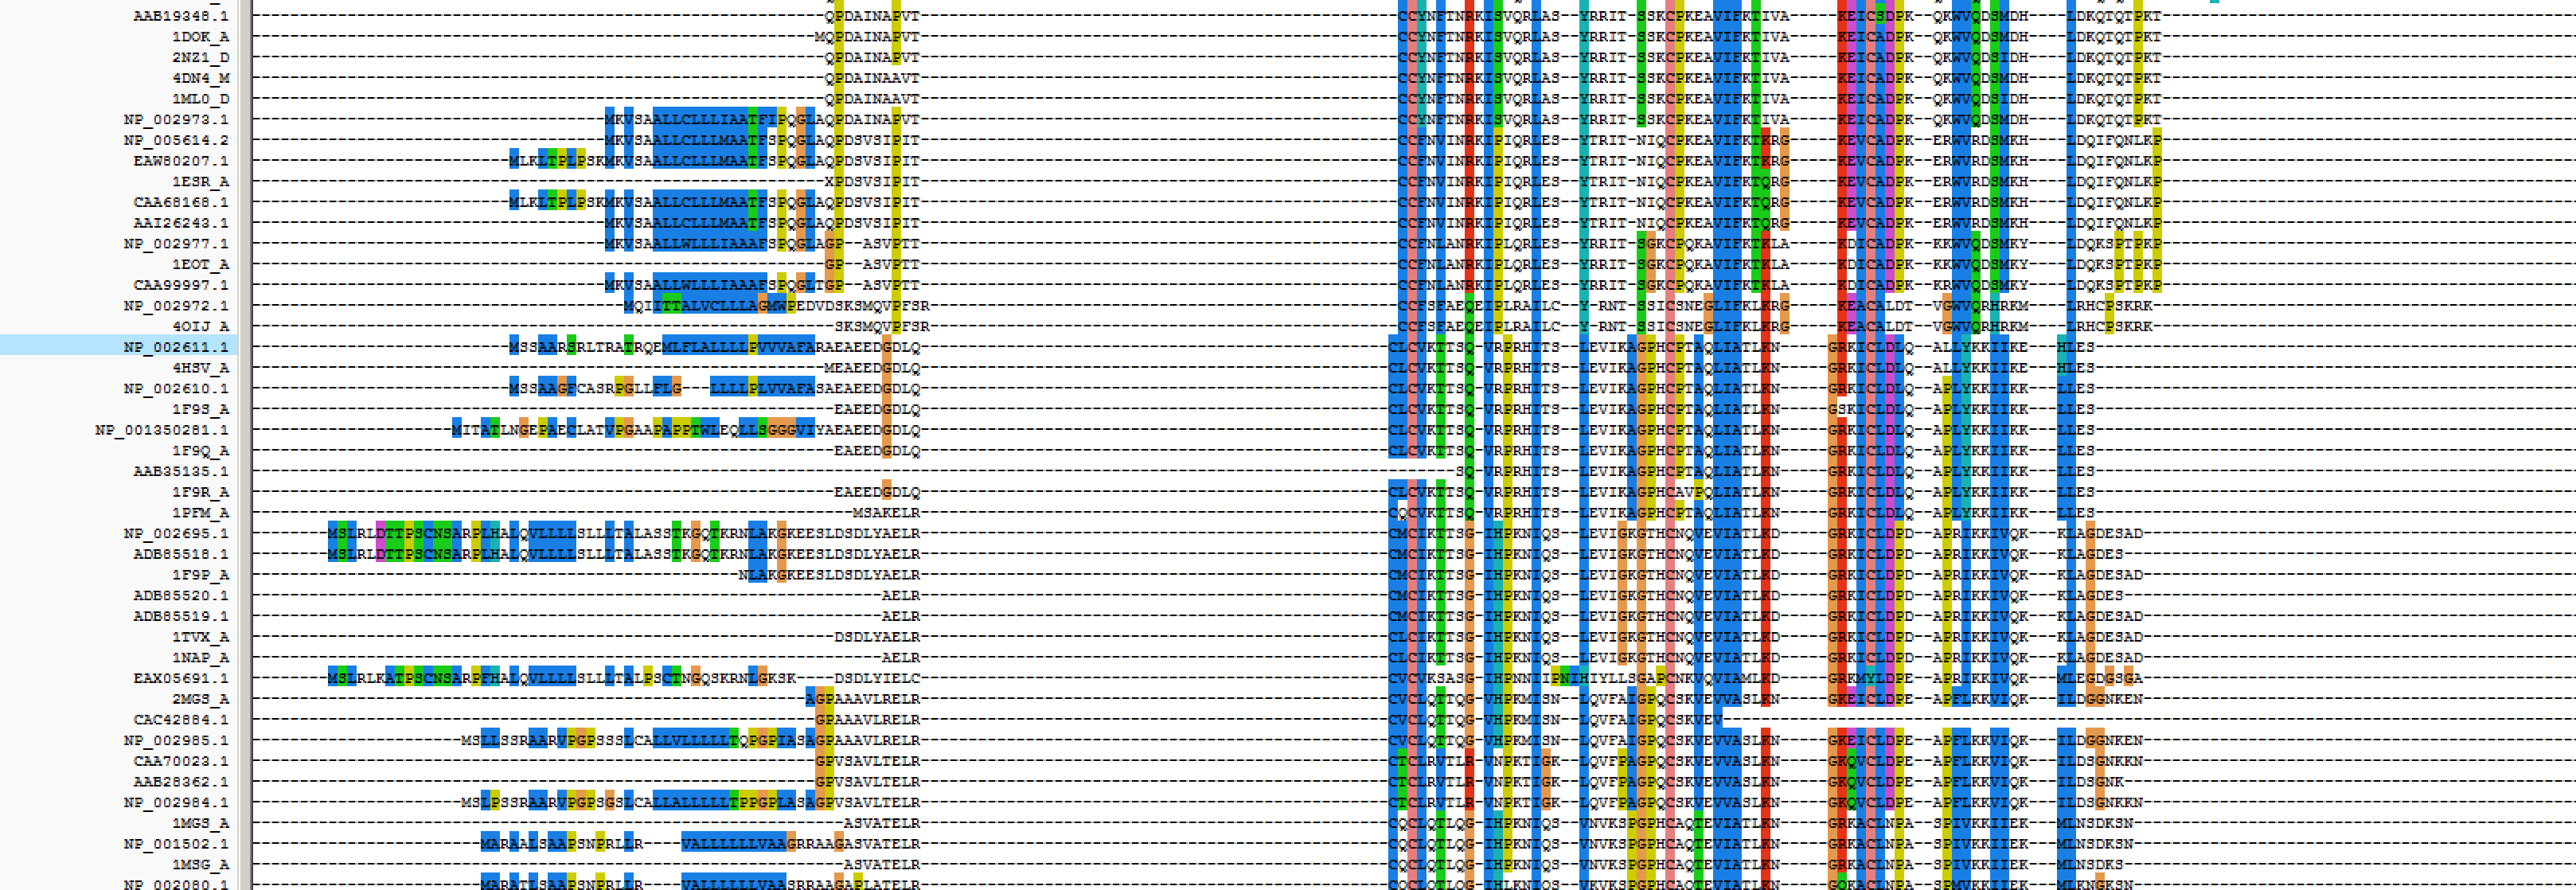
\includegraphics[width=1\textwidth]{image/MSA.png}
    \caption{MSA results}
    \label{HMCD3}
\end{figure}

According to the MSA results, A consensus pattern named C-X-C motif can be found in PF4 (NP\_002611.1). The hits indicated a conserved domain that classifies the PF4 into CXC family chemokine, which is a chemotactic factor that attracts neutrophils, basophils, and T-cells, but not monocytes, and is involved in neutrophil activation.

\begin{figure}[H]
    \centering
    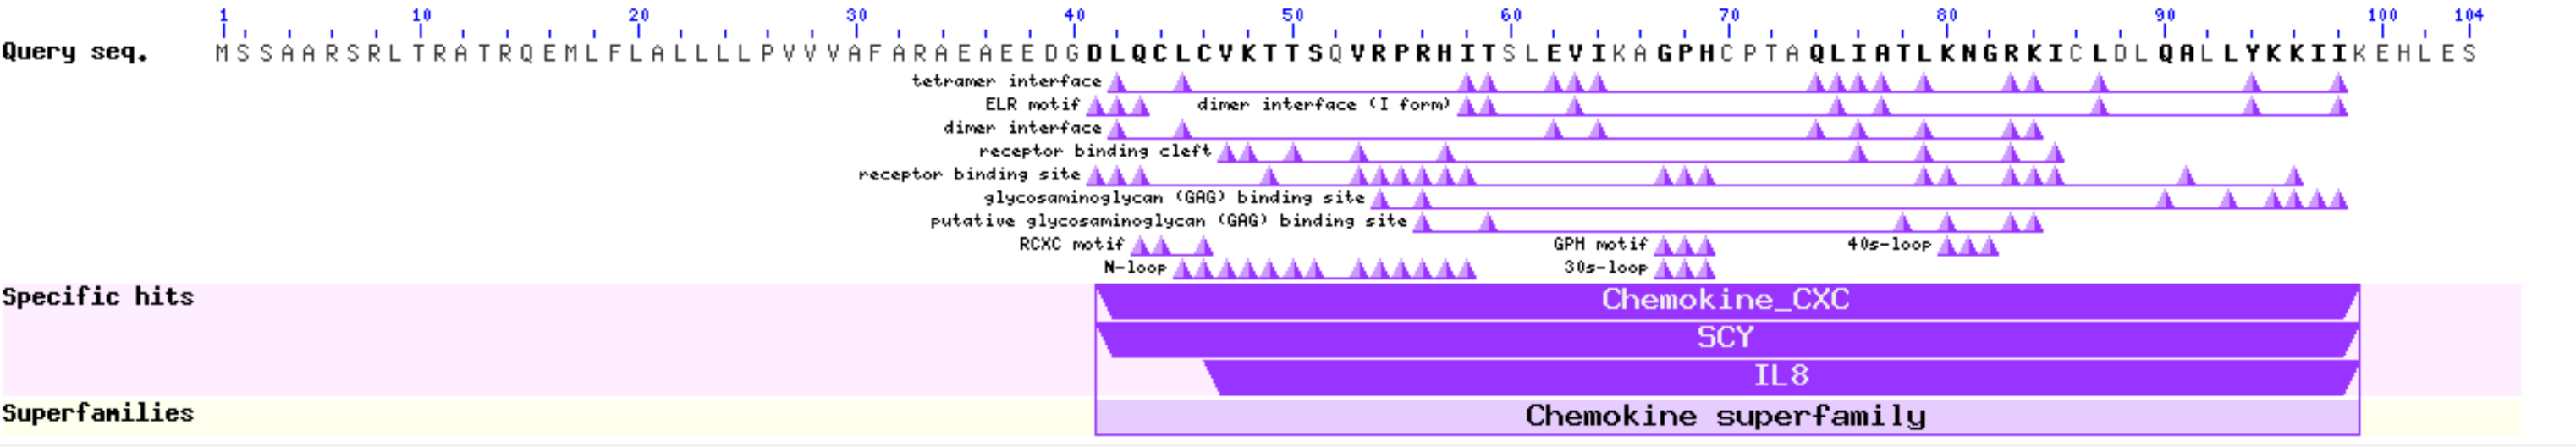
\includegraphics[width=1\textwidth]{image/PF4D.png}
    \caption{Conserved domain of Platelet factor 4}
    \label{HMCD3}
\end{figure}

Visualization of the PF4 is shown in the figure below. The purple colored part is the C-X-C motif.

\begin{figure}[H]
    \centering
    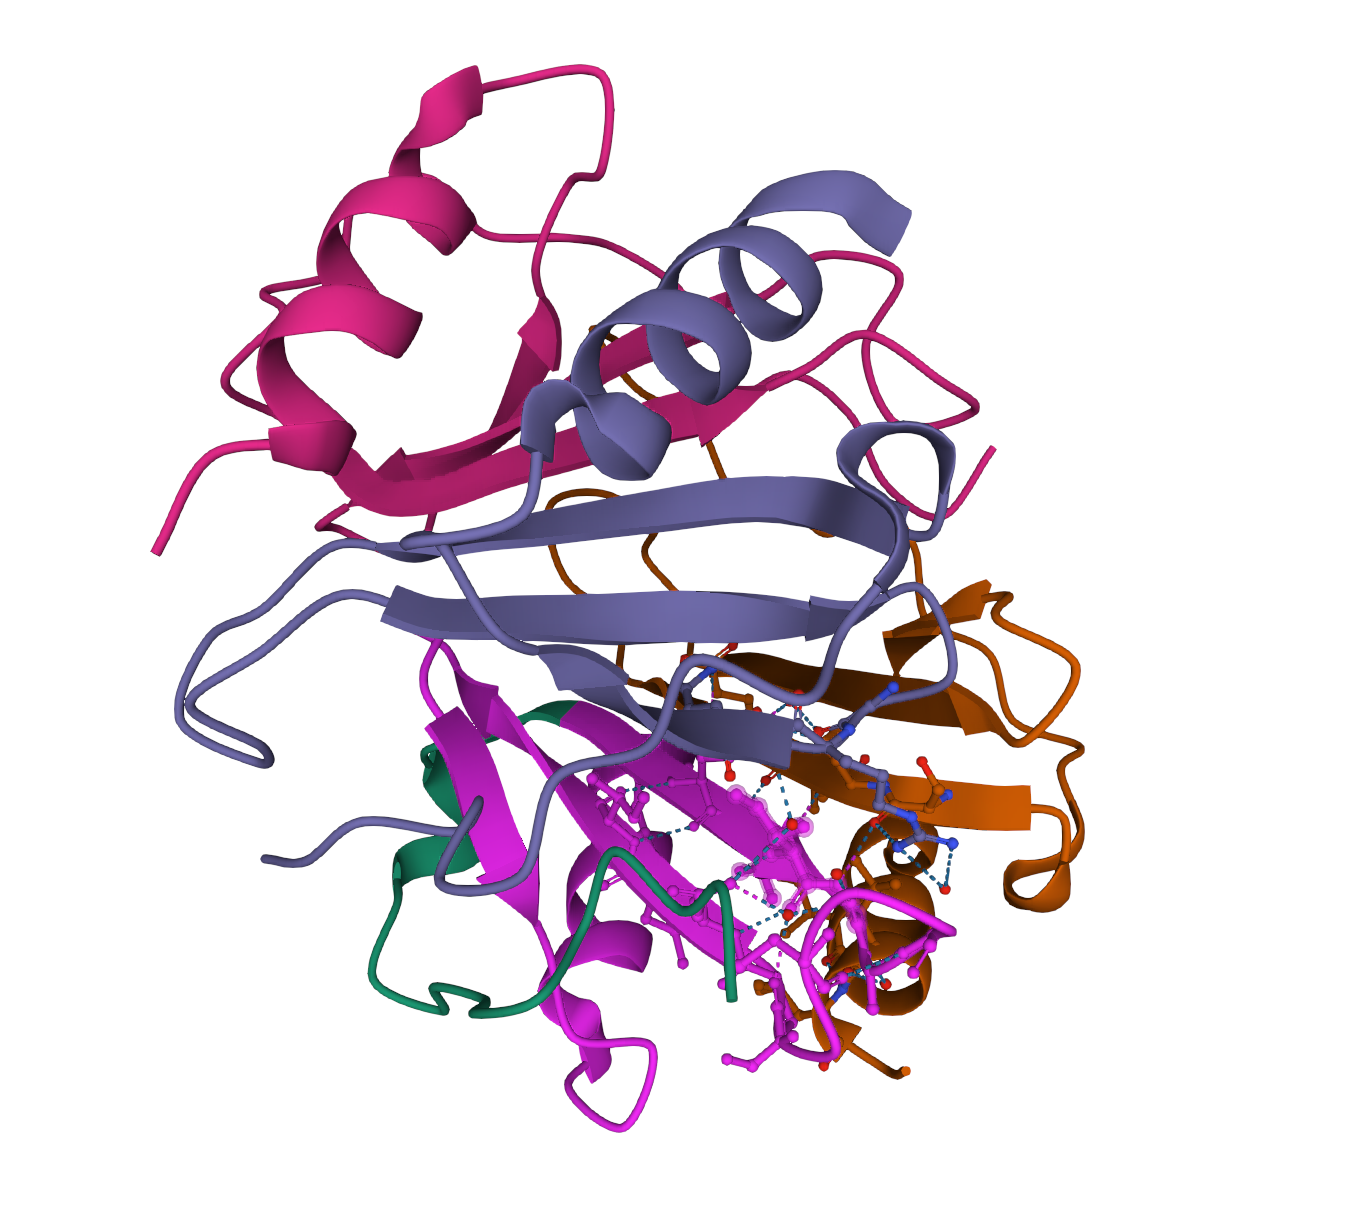
\includegraphics[width=1\textwidth]{image/PF43D2.png}
    \caption{Structure and Conserved domain of Platelet factor 4}
    \label{HMCD3}
\end{figure}

According to previous literature, platelet factor 4 (PF4) is a small cytokine belonging to the CXC chemokine family that is also known as chemokine (C-X-C motif) ligand 4 (CXCL4). This chemokine is released from alpha-granules of activated platelets during platelet aggregation, and promotes blood coagulation by moderating the effects of heparin-like molecules. Due to these roles, it is predicted to play a role in wound repair and inflammation. It is usually found in a complex with proteoglycan.\cite{fernandez2002structure}

\subsection{Platelet factor 4 and other CXC chemokine related genes are differently expressed in CD3+ T-cell of aplastic anemia patients.}

Among all the genes that are related to CXC chemokine family, 34 of them are measured on the micro array. There are 24 of the 34 relevant genes are down regulated in the patient group compared with the healthy control, while others are slightly up regulated. The differently expressed CXC chemokine related genes and their logFC values are demonstrated in the heat map below.

\begin{figure}[H]
    \centering
    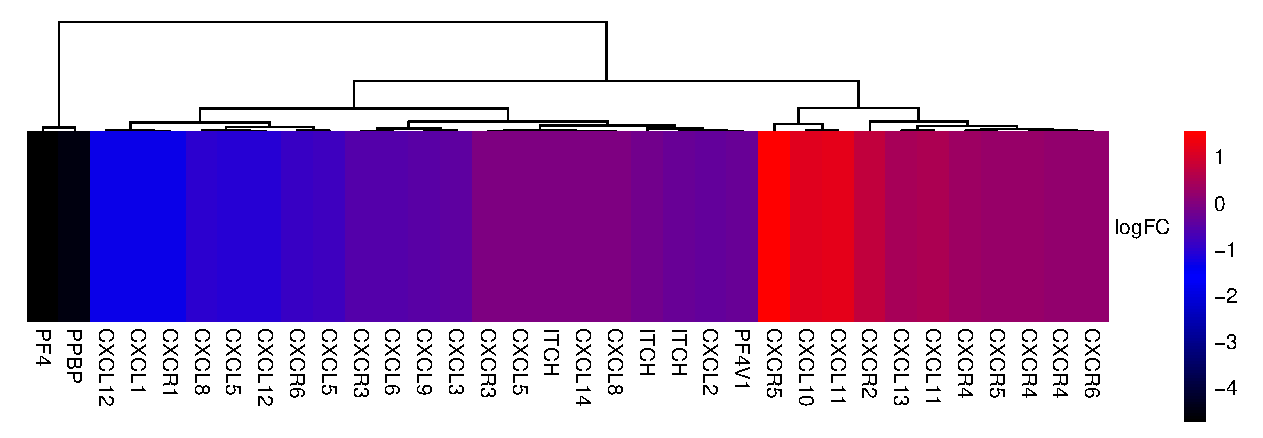
\includegraphics[width=1\textwidth]{image/CXCHM.eps}
    \caption{Structure and Conserved domain of Platelet factor 4}
    \label{HMCD3}
\end{figure}

\subsection{Platelet factor 4 is cleaved into a short form and binds heparin with high affinity.}

We queried the Nextprot database for more detailed information about Platelet factor 4. The platelet factor 4 has its signal peptide cut to form the mature protein, and the mature protein is cleaved into a short form, which can bind strongly to heparin. The figure below shows the sequence features of Platelet factor 4.

\begin{figure}[H]
    \centering
    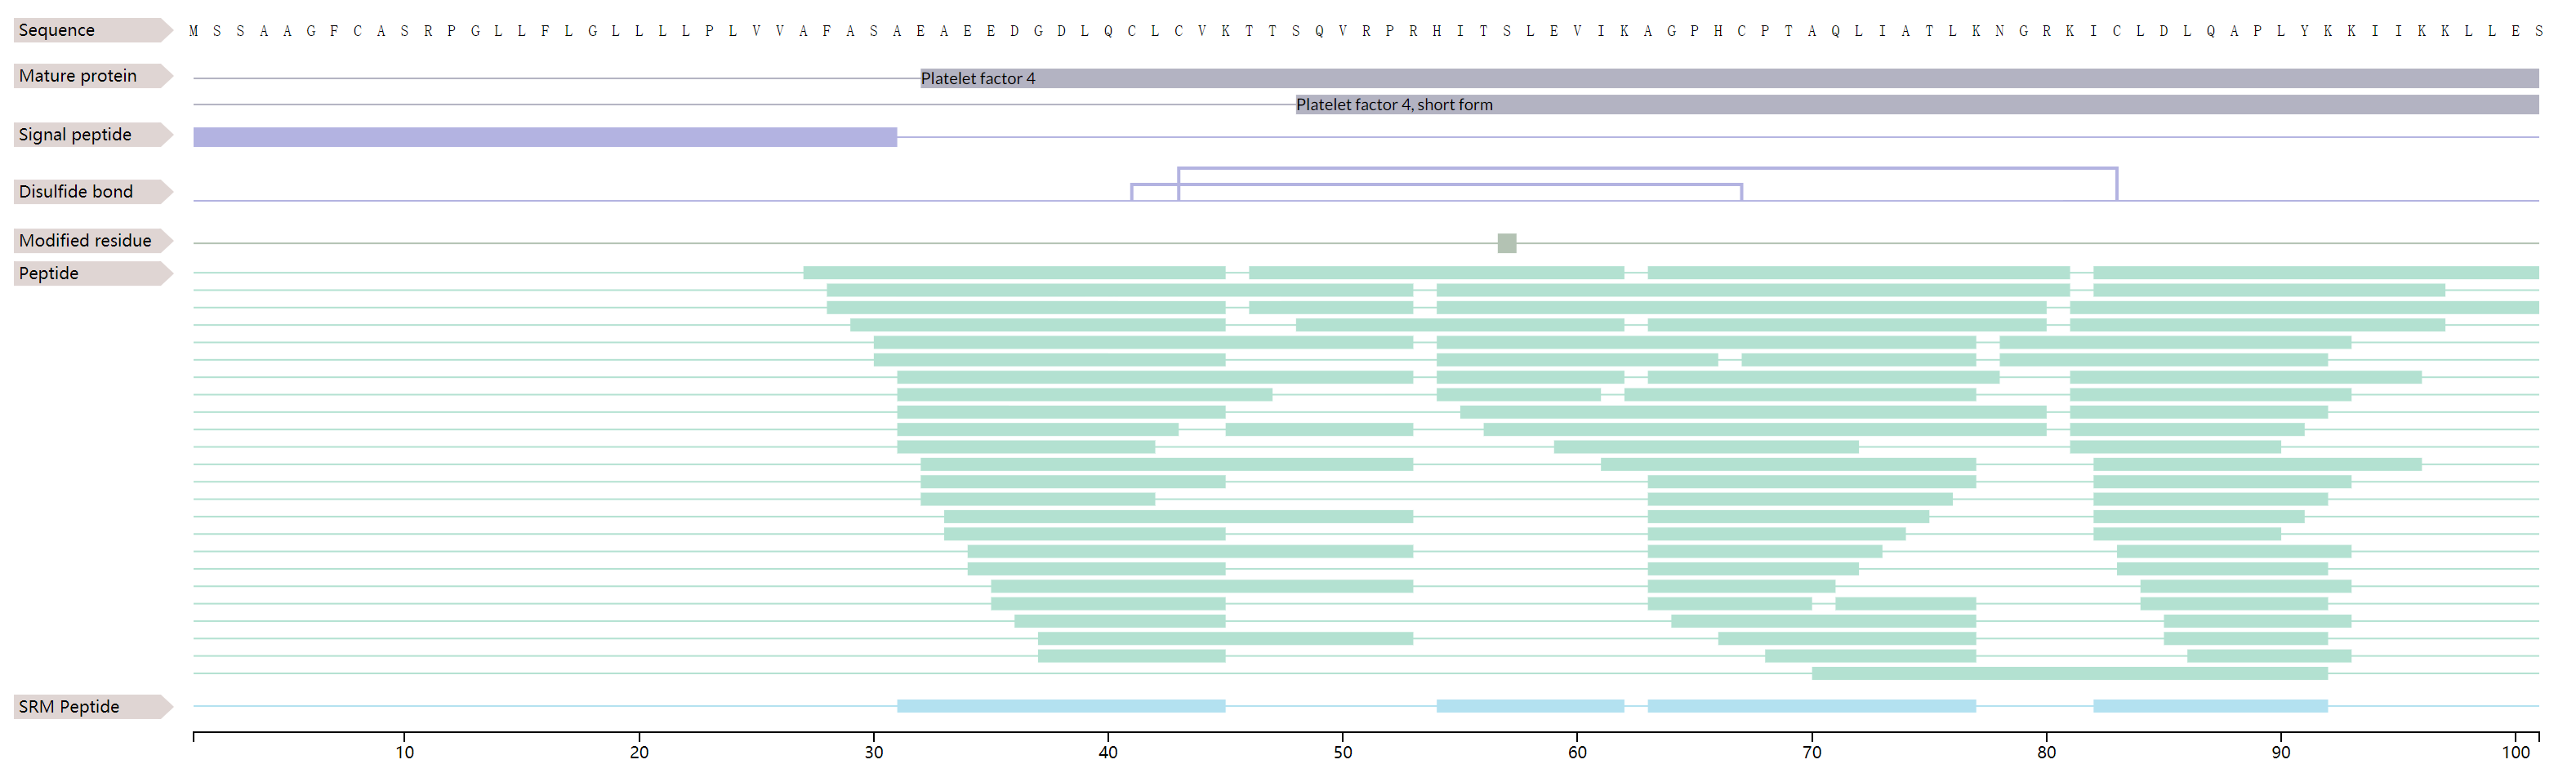
\includegraphics[width=1\textwidth]{image/PF4ISO.png}
    \caption{Sequence features of Platelet factor 4}
    \label{HMCD3}
\end{figure}

According to the GO annotation of platelet factor 4 in the database, it has high affinity to bind heparin, and we did a molecular docking to confirm this claim \textit{in silico}. 

The lowest energy conformation is shown in the figure below.

\begin{figure}[H]
    \centering
    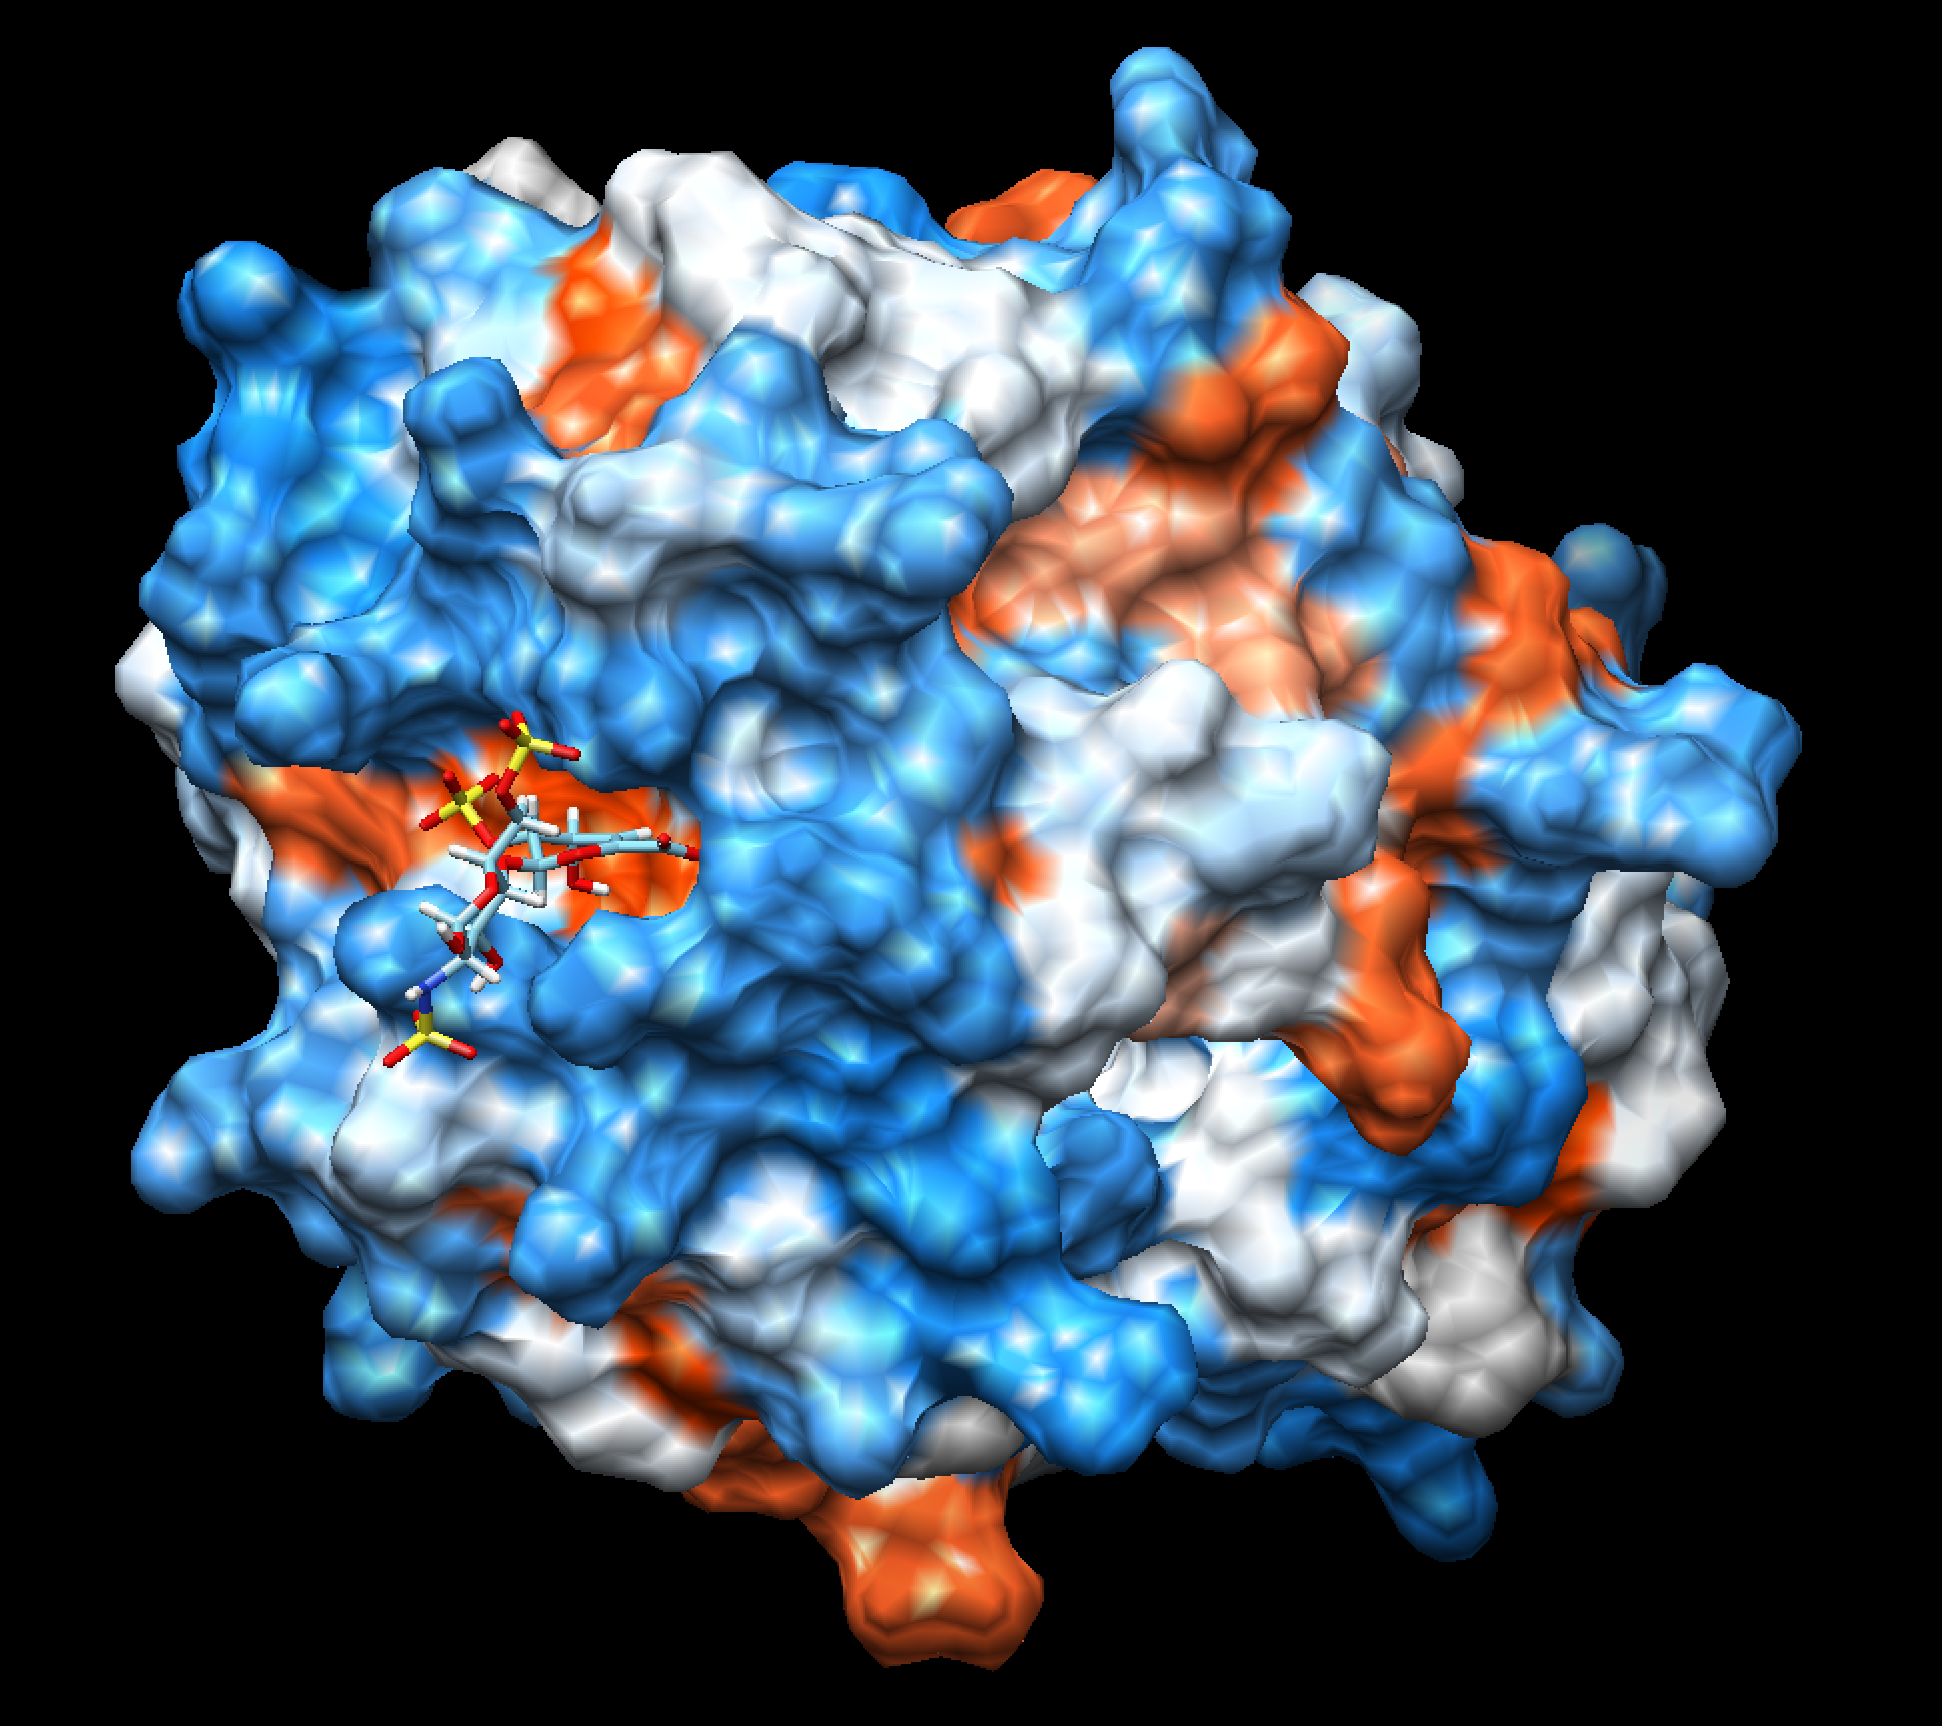
\includegraphics[width=0.7\textwidth]{image/DOCK.png}
    \caption{Lowest energy docking conformation}
    \label{HMCD3}
\end{figure}

\begin{lstlisting}
REMARK  Energy: -17.5306
REMARK  SimpleFitness: -17.5306
REMARK  FullFitness: -2058.942
REMARK  InterFull: -308.048
REMARK  IntraFull: 42.5802
REMARK  solvFull: -1990.93
REMARK  surfFull: 197.456
REMARK  extraFull: 0.0
REMARK  deltaGcompsolvpol: -1990.93
REMARK  deltaGcompsolvnonpol: 197.456
REMARK  deltaGprotsolvpol: -2104.32
REMARK  deltaGprotsolvnonpol: 195.666
REMARK  deltaGligsolvpol: -171.412
REMARK  deltaGligsolvnonpol: 12.8132
REMARK  deltaGvdw: -308.048
REMARK  deltaGelec: 0.0
REMARK  deltaG: -16.744253
REMARK  Cluster: 0
REMARK  ClusterRank: 0
\end{lstlisting}





\subsection{Immunosupressive agent Prednisone has less affinity to PF4, compared with heparin.}

We also docked commonly used immunosupressive agents like Prednisone, Cyclosporin and Tacrolimus, which are used in immunosupressive therapies, but they showed little affinity to PF4, compared with heparin.

The docking result of Prednisone is shown below.

\begin{figure}[H]
    \centering
    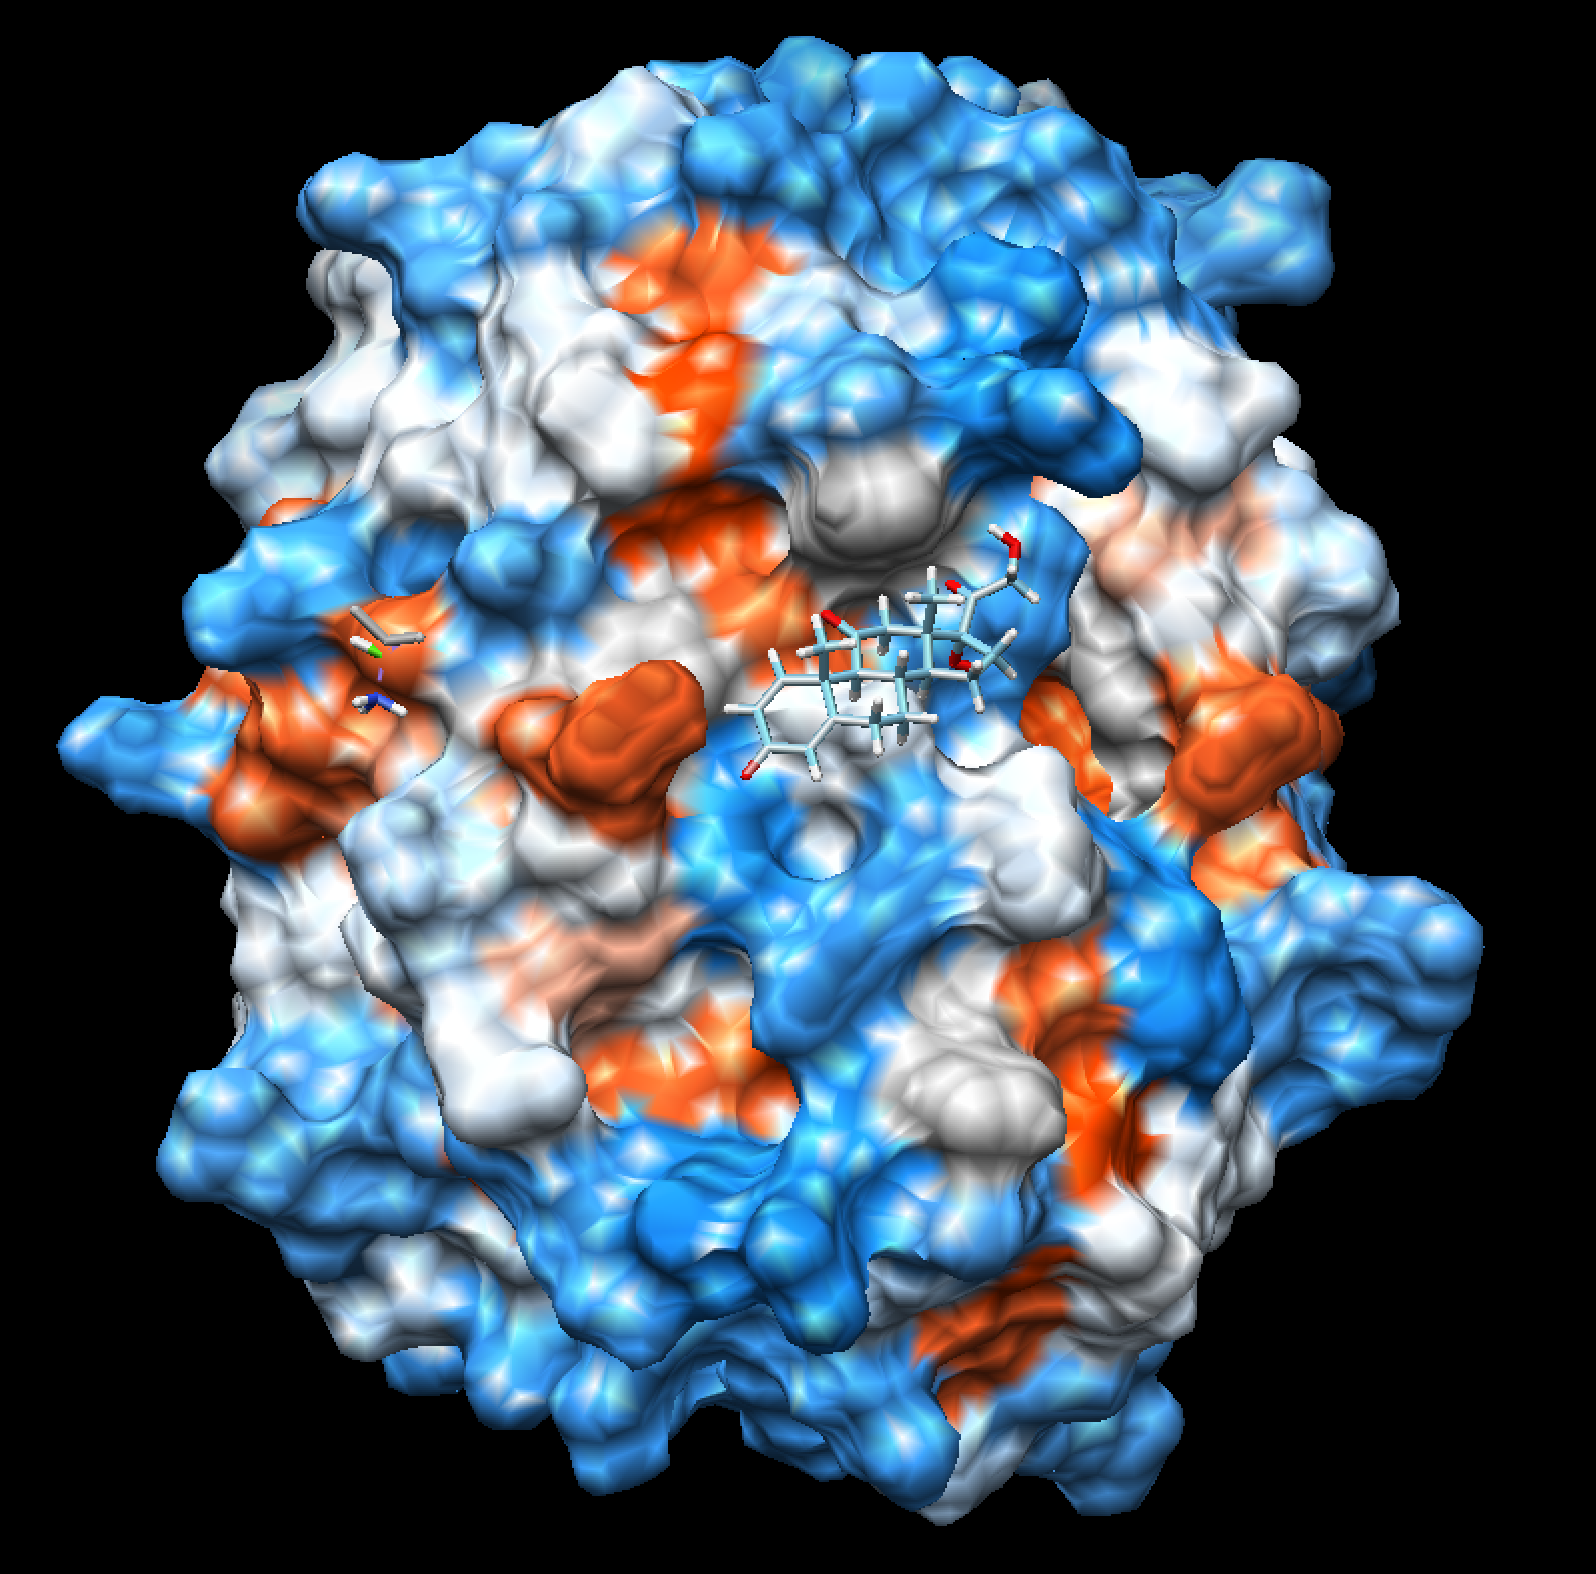
\includegraphics[width=0.7\textwidth]{image/DOCK2.png}
    \caption{Lowest energy docking conformation}
    \label{HMCD3}
\end{figure}

\begin{lstlisting}
REMARK  Energy: 26.0314
REMARK  SimpleFitness: 26.0314
REMARK  FullFitness: -1853.696
REMARK  InterFull: -36.5928
REMARK  IntraFull: 81.3677
REMARK  solvFull: -2095.95
REMARK  surfFull: 197.479
REMARK  extraFull: 0.0
REMARK  deltaGcompsolvpol: -2095.95
REMARK  deltaGcompsolvnonpol: 197.479
REMARK  deltaGprotsolvpol: -2104.32
REMARK  deltaGprotsolvnonpol: 195.666
REMARK  deltaGligsolvpol: -17.0954
REMARK  deltaGligsolvnonpol: 11.6588
REMARK  deltaGvdw: -36.5928
REMARK  deltaGelec: 0.0
REMARK  deltaG: -6.8246017
REMARK  Cluster: 0
REMARK  ClusterRank: 0

\end{lstlisting}

The optimal conformation in the figure above has -6.82 Estimated $\delta$G (kcal/mol) which is relatively weak. This indicates that Prednisone as an immunosupressive agent, may not be directly affecting the function of PF4.
